\section{Project outcomes}

\subsection{Concrete outcomes}

The project achieved two concrete outcomes:
\begin{itemize}
      \item \textbf{Electronic board}: The board was designed and assembled successfully. It includes an analog front end that extends the capabilities of the STM32's built in DAC and also includes features, such as the adc feedback and micro sd, that allows further experimentation.
      \item \textbf{Software drivers}: Two software drivers were developed, one for the DAC and one for the DMA. These allows to use the peripherals in a simple and efficient way.
\end{itemize}

\begin{figure}[h]
      \captionsetup[figure]{labelformat=empty}
      \centering
      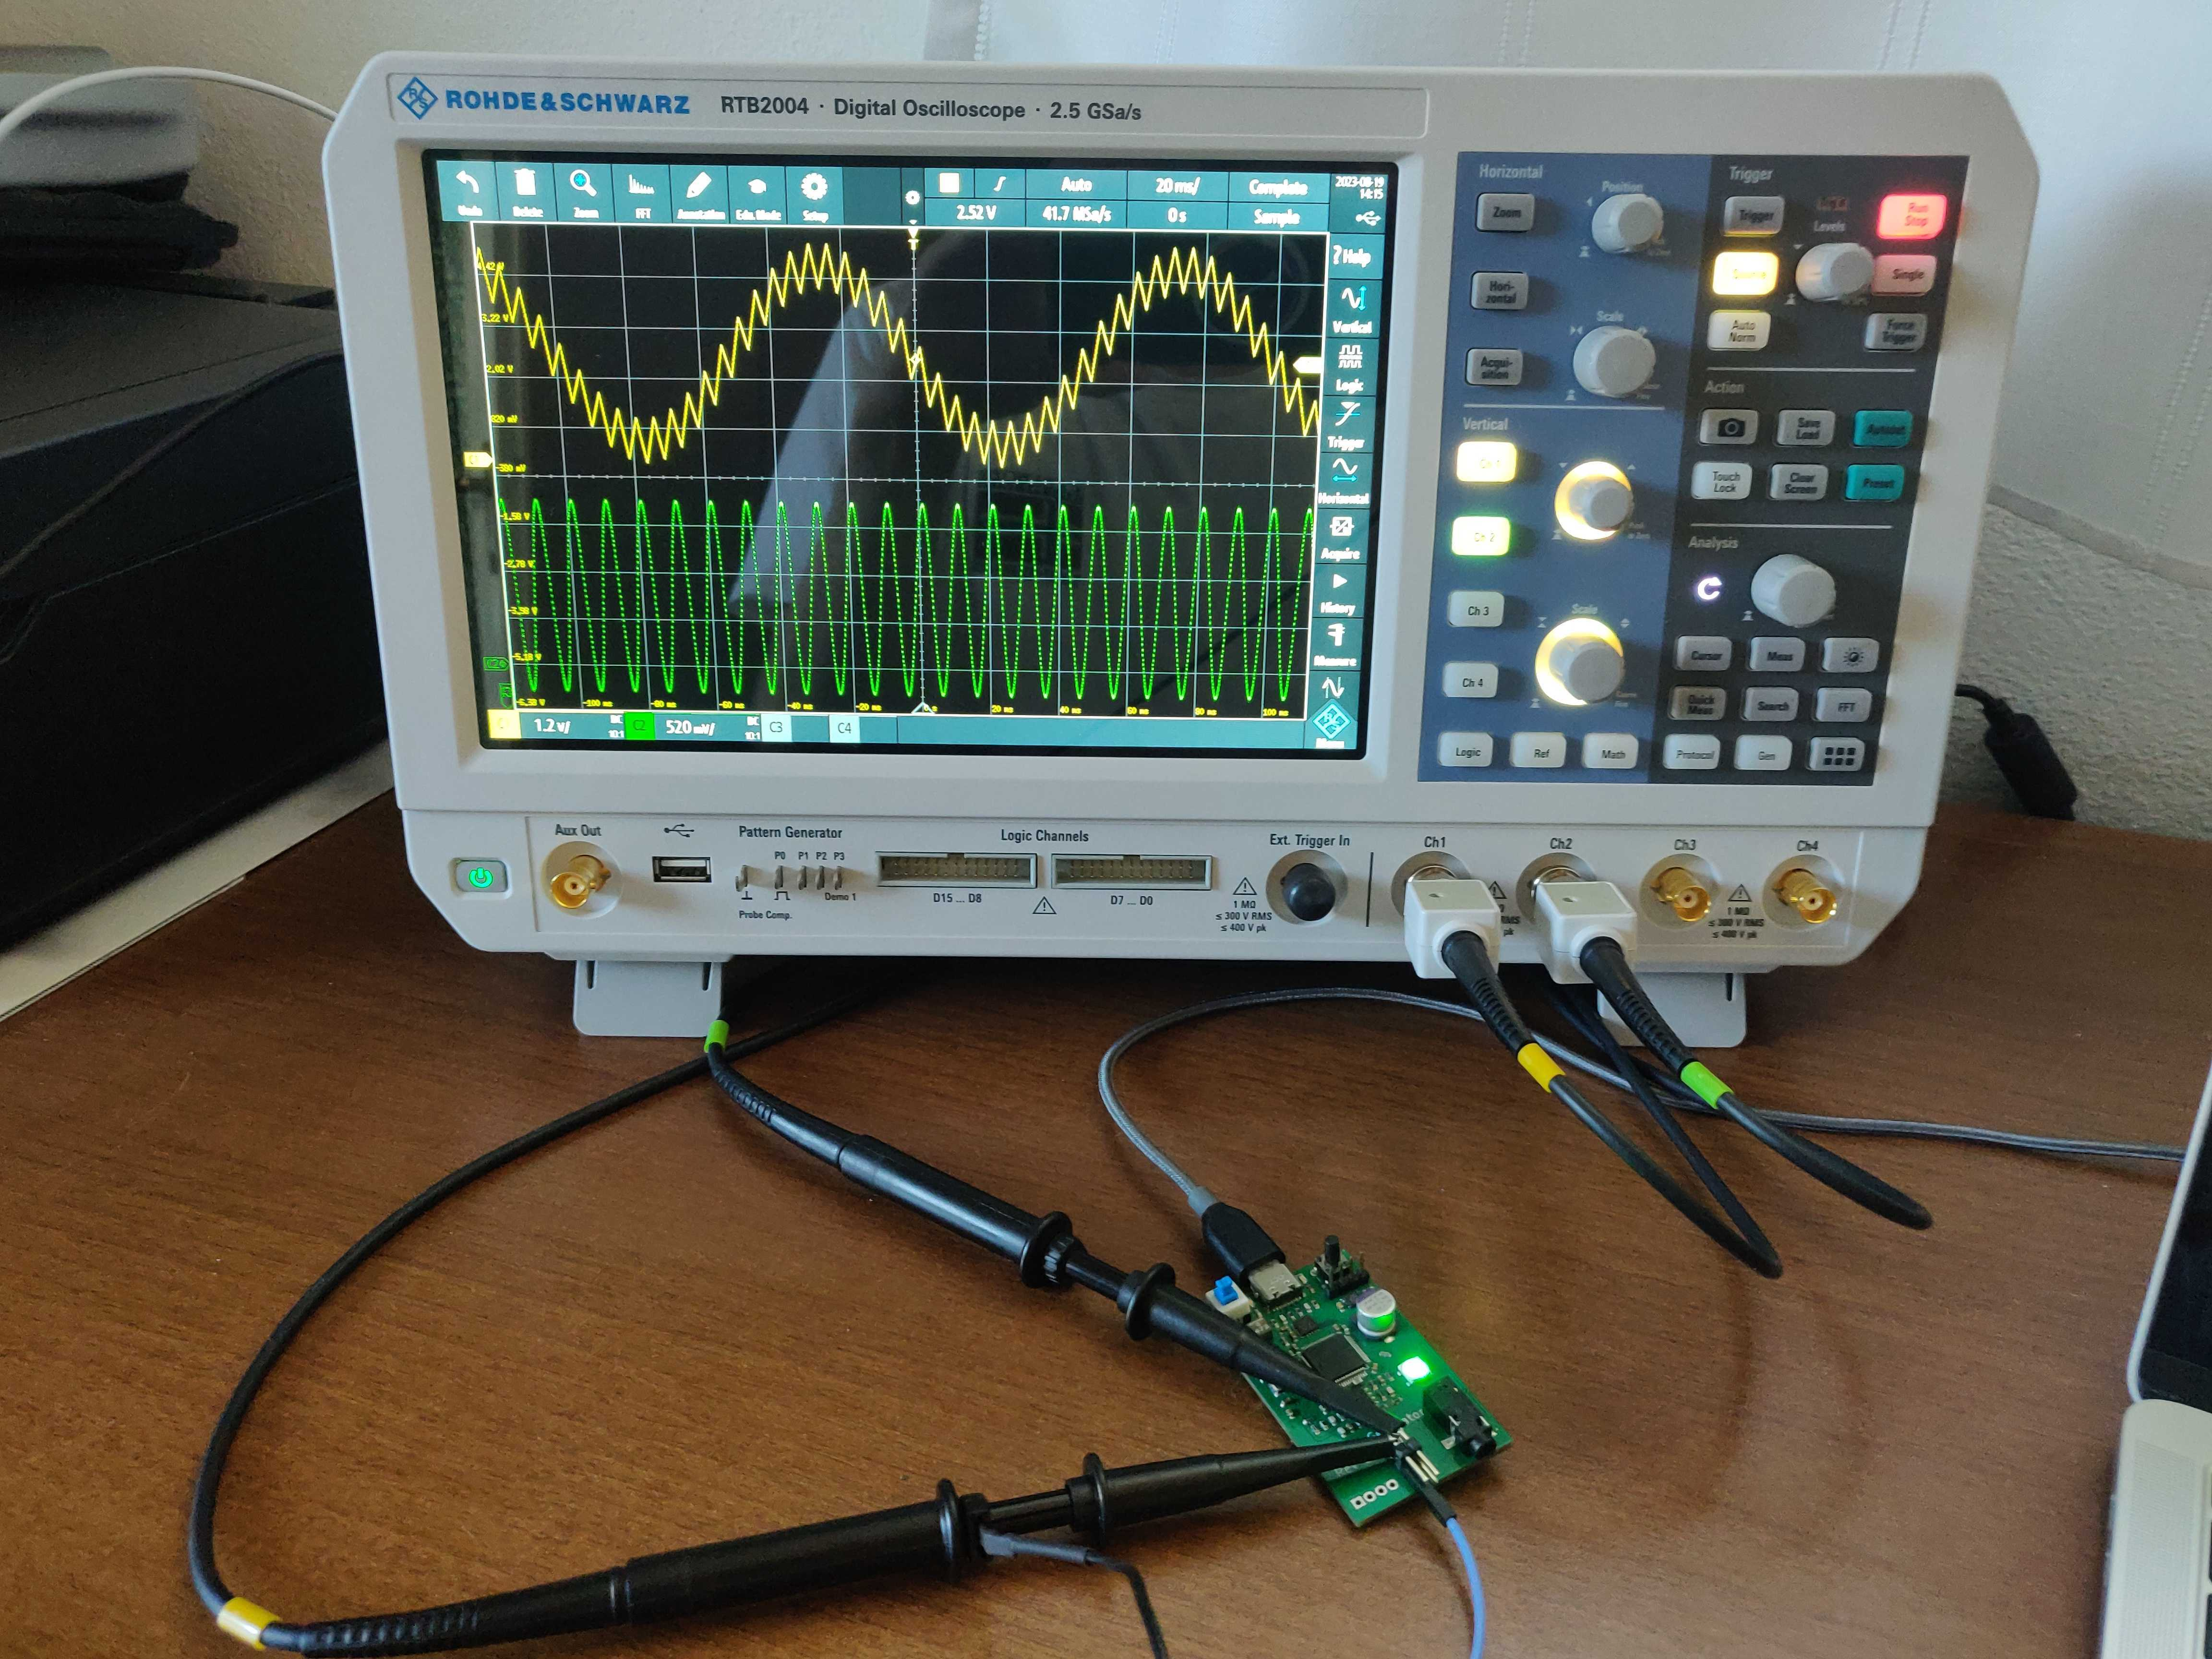
\includegraphics[width=0.5\textwidth]{graphics/device_with_oscilloscope.jpg}
      \caption{Signal Generator board hooked up to an oscilloscope}
\end{figure}

\subsection{Learning outcomes}

Developing both the hardware and the software allowed me not only to learn about the stm32 microcontroller and its peripherals, but also to learn about the whole process of designing and assembling a PCB.

\bigbreak

Particular effort went into the design of the board itself, selecting and sourcing the components and manually assembling the board. It was a challenge because, being my first time creating a complex PCB with a microcontroller, I was not well prepared. I had to learn about the different types of components, which were required for my design and which not. Some special takeaways were the importance of reading carefully the components datasheet, finding application notes to understand similar projects and learning how to design and order a PCB (with KiCad and JLCPCB).

\bigbreak

The assembly of the board was the most exciting part because I got to see my design come to life. I procured the necessary soldering equipment (solder paste, a hot plate, a hot air gun and a microscope) and I soldered the board first by distributing the solder paste with a stencil and then by heating the board with the hot plate for the top layer, and with the hot air gun for the bottom layer. I had to learn how to use the equipment and how to solder the different components.

\bigbreak

The software side was instead more akin to my previous experiences. I had already worked with microcontrollers and already used the Miosix operating system. However, I had never worked with the DMA peripheral. The most challenging aspects were to understand how the peripherals works by reading the reference manual and also find examples online which are hard to come by.

\subsection{Existing knowledge}

The most useful knowledge that helped me in this project came from 3 sources:
\begin{itemize}
      \item \textbf{Advanced Operating System}: In particular the parts on concurrency, thread programming and analysis of the features in the Miosix operating system.
      \item \textbf{Embedded Systems}: The course gave me a good understanding of the development process of a microcontroller based system, both for the design aspects and for the production processes involved.
      \item \textbf{Skyward Experimental Rocketry}: Most of the experience I had prior to this academic year was my involvement in the Skyward Experimental Rocketry team. Previously I was involved in the design and development of the software for the rocket. This year I also had the responsibility of managing the production of the avionic system as a whole, including the electronic part. This gave me a good opportunity to work on another project and the luck of knowing lots of talented teammates.
\end{itemize}

\subsection{Problems encountered}

The worst setback I faced was the board redesign. In the first version I used an STM32F103 which is a cheaper microcontroller that has not built in DAC! I realized this only after I had assembled the board and tried to use it. I had to adjust the schematic and the PCB in order to use the STM32F205 instead and reorder the board.

Once the board was ready I faced other problems during the development of the drivers but I managed to solve them without major issues. In this process the debugger was particularly useful to understand what was going on.
